

The theory of invariant observer design, based on the estimation error being invariant under the action of a matrix Lie Group, has recently been developed to Invariant EKF, which is applied to simultaneous localization and mapping in \cite{hartley2018contact}. This section derives a Left Invariant EKF to estimate the pose of the robot in the world frame using IMU and GPS measurements. The state is modelled as:

\begin{equation}
    X_{k} = 
    \begin{bmatrix}
    R_{k} & v_{k} & p_{k} \\
    0 & 1 & 0 \\
    0 & 0 & 1
    \end{bmatrix}
\end{equation}

where $R_{k} \in SO(3)$ is the orientation, $v_{k} \in \mathbb{R}^3$ is the linear velocity, and $p_{k} \in \mathbb{R}^3$ is the global position. IMU measurements are used for prediction and GPS measurements are used for correction.

In prediction, the angular acceleration ($w_{k} \in \mathbb{R}^3$) and linear acceleration $a_{k} \mathbb{R}^3$ obtained from the IMU are utilized as input to propagate the state mean using the following equations:

\begin{equation}
    R_{k+1}=R_{k}exp(\overline{\omega_{k}}\delta t)
\end{equation}

\begin{equation}
    v_{k+1}=v_{k}+R_{k}(\overline{\omega_{k}}\delta t)\overline{a_{k}}\delta t+g \delta t
\end{equation}

\begin{equation}
    p_{k+1}=p_{k}+v_{k}+R_{k}(\overline{\omega_{k}}\delta t)\overline{a_{k}}\delta t^{2}+(1/2)g \delta t
\end{equation}

The dynamics above does not consider the in-run bias in the accelerometer, given the fact that only $\pm$0.04 mg bias exists. In order to propagate the covariance, the adjoint operator is obtained as follows:

\begin{equation}
    Ad = 
    \begin{bmatrix}
    R & 0 & 0   \\
    (v)_{\times}R & R & 0  \\
    (p)_{\times}R & 0 & R 
    \end{bmatrix}
\end{equation}

where $()_{\times}$ denotes a $3 \times 3$ skew-symmetric matrix. 
The left-invariant error dynamics depend on the IMU inputs, which are assumed to be constant (following a zero-order hold) between $t_{k}$ and $t_{k+1}$. The state transition matrix for this specified case is determined as:

\begin{equation}
    \phi(t_{k+1},t_{k}) = exp(A \delta t)
\end{equation}

where $A$ is given as:

\begin{equation}
    A = 
    \begin{bmatrix}
    -\bar{\omega_{k}^{\wedge}} & 0 & 0  \\
    -\bar{a_{k}^{\wedge}} & -\bar{\omega_{k}^{\wedge}} & 0 \\
    0 & I & -\bar{\omega_{k}^{\wedge}}
    \end{bmatrix}
\end{equation}

In the correction step, GPS measurements are incorporated in the form:

\begin{equation}
    Y_{k}=\bar{X_{k}}b+V_{k}
\end{equation}

which can be written in the matrix form as:

\begin{equation}
    \begin{bmatrix}
    y_{k} \\
    0 \\
    1
    \end{bmatrix}
    =
    \begin{bmatrix}
    \bar{R_{k}} & \bar{v_{k}} & \bar{p_{k}} \\
    0 & 1 & 0 \\
    0 & 0 & 1
    \end{bmatrix}
    \begin{bmatrix}
    0\\
    0\\
    1
    \end{bmatrix}
    +
    \begin{bmatrix}
    v_{k}\\
    0\\
    0
    \end{bmatrix}
\end{equation}

Using the Left-Invariant EKF equations, H is obtained as:

\begin{equation}
H = 
    \begin{bmatrix}
    0 & 0 & I_{3}
    \end{bmatrix}
\end{equation}

The belief mean ($\bar{X_{t_{k}}^+}$) and covariance ($\bar{P_{t_{k}}^+}$) are then updated with the following equations: 

\begin{equation}
\bar{X}_{t_{k}}^+ = \bar{X}_{t_{k}}^+ 
exp(L_{tk} (\bar{X}_{t_{k}}^{-1}Y_{t_k}-b) )
\end{equation}

\begin{equation}
\bar{P}_{t_{k}}^+ = (I - L_{t_k} H )P_{t_k}(I - L_{t_k} H )^T
+L_{t_k}\bar{N}_{k}L_{t_k}^T
\end{equation}

where 
\begin{equation}
L_{t_k} = P_{t_{k}} H^T S^{-1}
\end{equation}

\begin{equation}
S = HP_{t_k} H^T + \bar{N}_{k}
\end{equation}

The IMU measurements are sampled at 100 Hz, while the GPS measurements are sampled at 10 Hz. We resampled the IMU measurements to 10Hz to match the frequency of GPS measurements and reduce filter runtime.

Although the InEKF algorithm deals with 3D data and states, our implementation focuses only on the x-y position of the robot. Figure \ref{fig:imugps-20s} and Figure \ref{fig:imugps-40s} show the first 20 and 40 seconds of the path, respectively. Figure \ref{fig:imugps-40s} shows the results from the Left-InEKF filter without the prediction step, which means only GPS measurements are used. Both plots show that the results from the filter match accordingly with the GPS data with a maximum difference less than 0.5 meter. The validity of the Left-InEKF filter is proved.

\begin{figure}[hbt!]
    \centering
    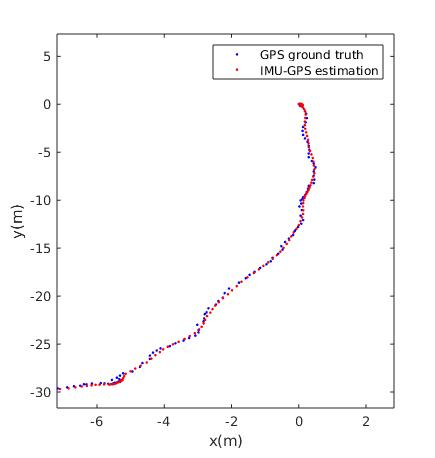
\includegraphics[width = 0.5\linewidth]{media/Starting_results.jpg}
    \caption{Comparison between the IMU-GPS estimation and GPS ground truth in the first 20 secs of data collection}
    \label{fig:imugps-20s}
\end{figure}

\begin{figure}[hbt!]
    \centering
    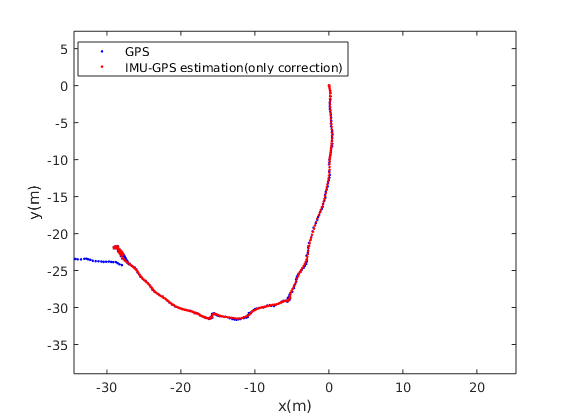
\includegraphics[width = 0.8\linewidth]{media/OnlyGPS.png}
    \caption{Comparison between the filter estimation using only the GPS correction and GPS ground truth in the first 40 secs of data collection}
    \label{fig:imugps-40s}
\end{figure}

Figure \ref{fig:complete_IMUGPS_result} compares the pose estimation from the filter with the ground truth. The starting position of the ground truth is set at the origin.

\begin{figure}[hbt!]
    \centering
    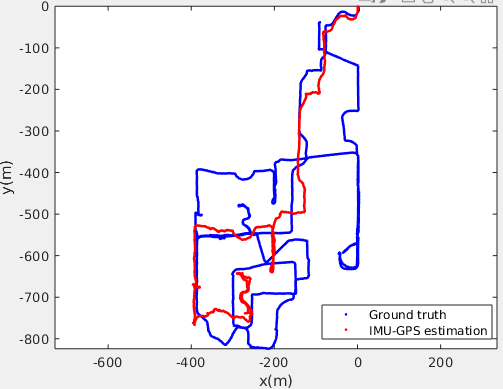
\includegraphics[width = 0.8\linewidth]{media/Complete_InEKF_Result.png}
    \caption{Comparison between the IMU-GPS estimation and the ground truth. About half of the dataset has been processed by the LI-EKF.}
    \label{fig:complete_IMUGPS_result}
\end{figure}

